%%%%%%%%%%%%%%%%%%%%%%%%%%%%%%%%%%%%%%%%%%%%%%%%%%%%%
% Author: [Francesco Giraudo]
% Date: 2025-05-03
% Description: [Exercise Set 2 - Computational Finance]
%%%%%%%%%%%%%%%%%%%%%%%%%%%%%%%%%%%%%%%%%%%%%%%%%%%%%

\documentclass{article}
\usepackage[english]{babel}
\usepackage{amsfonts}
\usepackage{amsmath} 
\usepackage{amssymb}
\usepackage{graphicx}
\usepackage{geometry}
\usepackage{mdframed}
\usepackage{booktabs}

\renewcommand{\thesubsection}{\thesection.\alph{subsection}} % Letter for subsections

% Set custom margins
\geometry{
  top=0.5in,
  bottom=0.75in,
  left=0.78in,
  right=0.78in
}

% Eliminate paragraph indentation
\setlength{\parindent}{0pt}

\title{Computational Finance - Exercise set 02}
\author{Francesco Giraudo \\ \small{Vrije Universiteit} \\ {\small\texttt{f.giraudo@student.vu.nl}}}
\date{7 May 2025}

\begin{document}

\maketitle

\vspace{-1cm}

\section{Exercise 1}

\subsection{}


European option values under a Black-Scholes model with a time-dependent volatility function $\sigma(t)$ are identical to the corresponding option values obtained by a log-transformed model based on the equivalent constant volatility $\sigma_*$. This equivalence arises from matching the first two moments of the log-price distribution

\begin{align*}
\mathbb{E}[\log S(T)] &= \log S_0 + \int_0^T \left(r - \frac{1}{2} \sigma^2(t)\right) dt = \log S_0 + \left(r - \frac{1}{2} \sigma_*^2\right) T \\
\mathrm{Var}[\log S(T)] &= \int_0^T \sigma^2(t) dt = \sigma_*^2 T.
\end{align*}

This ensures identical marginal distributions for the two processes at maturity, although their transitional distributions may differ. The equivalent constant volatility $\sigma_*$ is given by:
\begin{equation}
\sigma_*^2 = \frac{1}{T} \int_0^T \left(0.6 - 0.2 e^{-1.5t}\right)^2 dt = \frac{1}{T}\left(0.36T + \frac{0.24}{1.5}(1 - e^{-1.5T}) - \frac{0.04}{3}(1 - e^{-3T})\right)
\end{equation}
which simplifies to:
\begin{equation}
\sigma_* = \sqrt{0.36 + \frac{0.16}{T}(1 - e^{-1.5T}) - \frac{0.04}{3T}(1 - e^{-3T})}
\label{eq:sigma_star}
\end{equation}

\begin{figure}[h!]
    \centering
    \begin{minipage}{0.42\linewidth}
        \centering
        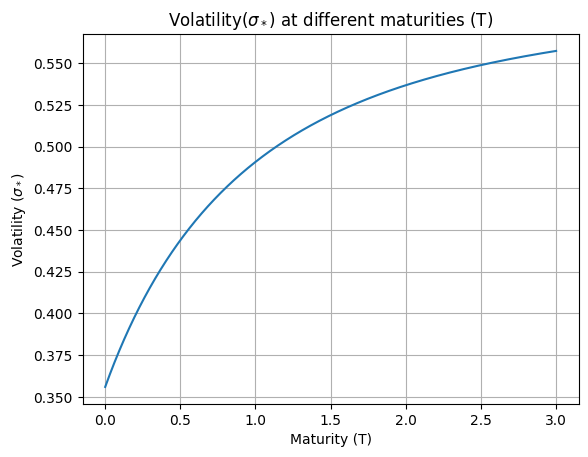
\includegraphics[width=1.05\linewidth]{Exercise_set_02/img/01A_Volatility.png}
        \caption{Value of $\sigma_*$ for different maturities T}
        \label{fig:volatility}
    \end{minipage}%
    \hfill
    \begin{minipage}{0.58\linewidth}
        \centering
        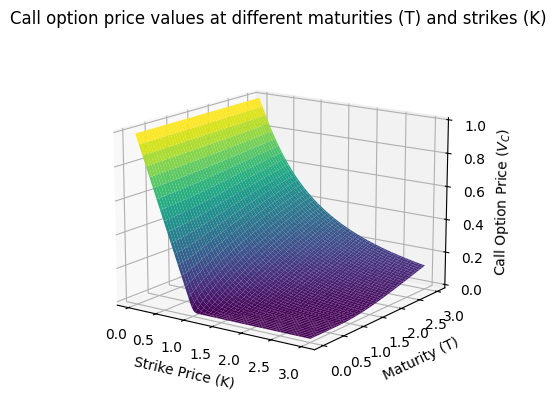
\includegraphics[width=0.8\linewidth]{Exercise_set_02/img/01A_Vc.png}
        \caption{$V_C$ vlue for different maturities T and strikes K}
        \label{fig:vc}
    \end{minipage}
\end{figure}
The European call option price at time $t=0$ under this GBM model with equivalent constant volatility $\sigma_*$ is obtained via the standard Black–Scholes formula using:
\begin{equation}
V_C(S_0,T,K,r,\sigma_*) = S_0 \Phi(d_1) - Ke^{-rT}\Phi(d_2)
\end{equation}
where
\begin{align*}
d_1 = \frac{\ln\frac{S_0}{K} + \left(r + \frac{\sigma_*^2}{2}\right)T}{\sigma_*\sqrt{T}} \qquad \qquad
d_2 = d_1 - \sigma_*\sqrt{T}
\end{align*}
with $\Phi(x)$ representing the cumulative distribution function (CDF) of the standard normal distribution $\mathcal{N}(0,1)$.

In Figure \ref{fig:vc} a plot of the values of the call option for different strikes and maturities.

\subsection{}
\newpage

\section{Exercise 2}

\subsection{}
Consider the stochastic differential equation:
\begin{equation*}
    dS(t) = \gamma \sqrt{S(t)} \, dW(t), \quad S(0) = s_0 > 0.
\end{equation*}

Let $X(t) = g(t, S(t)) := \frac{2}{\gamma} \sqrt{S(t)}$. Applying Itô's formula for a function $g(t, S)$, with $S(t)$ governed by an SDE, gives:
\begin{equation*}
    dg(t, S(t)) = \frac{\partial g}{\partial t} \, dt + \frac{\partial g}{\partial S} \, dS(t) + \frac{1}{2} \frac{\partial^2 g}{\partial S^2} \, (dS(t))^2.
\end{equation*}

For $g(t, S) = \frac{2}{\gamma} \sqrt{S}$, the partial derivatives are:
\begin{equation*}
    \frac{\partial g}{\partial t} = 0, \quad \frac{\partial g}{\partial S} = \frac{1}{\gamma \sqrt{S}}, \quad \frac{\partial^2 g}{\partial S^2} = -\frac{1}{2 \gamma S^{3/2}}.
\end{equation*}

Given $dS(t) = \gamma \sqrt{S(t)} \, dW(t)$ and $(dS(t))^2 = \gamma^2 S(t) \, dt$, substitution into Itô's formula yields:
\begin{align*}
    dX(t) &= \frac{1}{\gamma \sqrt{S(t)}} \cdot \gamma \sqrt{S(t)} \, dW(t)
           + \frac{1}{2} \cdot \left(-\frac{1}{2 \gamma S(t)^{3/2}}\right) \cdot \gamma^2 S(t) \, dt \\
          &= dW(t) - \frac{1}{2 X(t)} \, dt.
\end{align*}

The process $X(t)$ satisfies the stochastic differential equation:
\begin{equation*}
    dX(t) = dW(t) - \frac{1}{2 X(t)} \, dt,
\end{equation*}
which corresponds to a Bessel process of dimension $1$.

Therefore, $X(t)^2$ is a squared Bessel process and since $S(t) = \left( \frac{\gamma}{2} X(t) \right)^2$, it follows that $S(T)$ is distributed as:
\begin{equation*}
    S(T) \sim \frac{\gamma^2}{4} \cdot \chi^2_1(\lambda), \quad \lambda = X(0)^2 = \left( \frac{2}{\gamma} \sqrt{s_0} \right)^2 = \frac{4 s_0}{\gamma^2}.
\end{equation*}

The characteristic function of a scaled noncentral chi-squared variable $Y = c \cdot \chi^2_\nu(\lambda)$ is:
\begin{equation*}
    \phi_Y(u) = (1 - 2iuc)^{-\nu/2} \exp\left( \frac{iuc\lambda}{1 - 2iuc} \right).
\end{equation*}

Here, $c = \frac{\gamma^2}{4}$, $\nu = 1$, and $\lambda = \frac{4 s_0}{\gamma^2}$, so the characteristic function of $S(T)$ becomes:
\begin{align*}
    \phi_{S(T)}(u)
    &= \left(1 - 2i u \cdot \frac{\gamma^2}{4} \right)^{-1/2}
    \exp\left( \frac{i u \cdot \frac{\gamma^2}{4} \cdot \frac{4 s_0}{\gamma^2}}{1 - 2i u \cdot \frac{\gamma^2}{4}} \right) \\
    &= \left(1 - \frac{i u \gamma^2}{2} \right)^{-1/2}
    \exp\left( \frac{i u s_0}{1 - \frac{i u \gamma^2}{2}} \right).
\end{align*}

\newpage

\section{Exercise 3}


In this experiment, the price of a European call option was computed under a geometric Brownian motion (GBM) with time-dependent volatility
\[
\sigma(t) = 0.6 - 0.2e^{-1.5t}
\]
and a piecewise constant interest rate given by
\[
r(t) = 0.05 \cdot \mathbf{1}_{\{t < 2\}} + 0.08 \cdot \mathbf{1}_{\{t \geq 2\}}.
\]


The Euler scheme used the discretization:
\[
S_{t+\Delta t} = S_t + r(t) S_t \Delta t + \sigma(t) S_t (W_{t+\Delta t} - W_t)
\]
and the Milstein scheme applied:
\[
S_{t+\Delta t} = S_t + r(t) S_t \Delta t + \sigma(t) S_t (W_{t+\Delta t} - W_t) + \frac{1}{2} \sigma^2(t) S_t \left((W_{t+\Delta t} - W_t)^2 - \Delta t\right).
\]

\begin{table}[h!]
\centering
\label{tab:euler}
\begin{tabular}{|c|cccc|}
\hline
\textbf{Paths} & \textbf{m=50} & \textbf{m=100} & \textbf{m=200} & \textbf{m=400} \\
\hline
1000    & 0.49809 & 0.46843 & 0.38633 & 0.37968 \\
10000   & 0.38844 & 0.40604 & 0.36678 & 0.35852 \\
100000  & 0.36848 & 0.36646 & 0.36517 & 0.36358 \\
\hline
\end{tabular}
\caption{Euler scheme: option prices for different \(N\) and \(m\)}
\end{table}

\begin{table}[h!]
\centering
\label{tab:milstein}
\begin{tabular}{|c|cccc|}
\hline
\textbf{Paths} & \textbf{m=50} & \textbf{m=100} & \textbf{m=200} & \textbf{m=400} \\
\hline
1000    & 0.49545 & 0.46906 & 0.38049 & 0.37958 \\
10000   & 0.38021 & 0.40226 & 0.36407 & 0.35829 \\
100000  & 0.36434 & 0.36393 & 0.36382 & 0.36278 \\
\hline
\end{tabular}
\caption{Milstein scheme: option prices for different \(N\) and \(m\)}
\end{table}

The results in Tables~\ref{tab:euler} and~\ref{tab:milstein} demonstrate consistent convergence of the estimated European call option prices as both \(N\) and \(m\) increase. The Milstein method shows a marginal advantage in terms of stability and reduced numerical error, consistent with its inclusion of higher-order terms in the stochastic Taylor expansion.

\bigskip

Additionally, barrier options were computed using the same framework with barrier level \(B = 1.5\) and strike \(K = 1.6\), as requested. Given the initial asset price \(S_0 = 1\), which is below the barrier, the up-and-out option is deactivated immediately and consistently returns a value of zero. On the other hand, the up-and-in option yields results identical to the European option. This is because \(S_0 = 1 < B = 1.5 < K = 1.6\), so the only paths contributing to a non-zero payoff are those where the final price exceeds the strike, which necessarily implies that the barrier has been crossed.


\newpage

\section{Exercise 4}

Let $S_1(t)$ and $S_2(t)$ be two correlated geometric Brownian motions under the risk-neutral measure $\mathbb{Q}$, defined by:

\begin{equation*}
dS_1(t) = r S_1(t)\,dt + \sigma_1 S_1(t)\,dW_1(t), \quad
dS_2(t) = r S_2(t)\,dt + \sigma_2 S_2(t)\,dW_2(t),
\end{equation*}

with initial values $S_1(0) = S_2(0) = S_0$, volatilities $\sigma_1 = 0.4$, $\sigma_2 = 0.15$, constant interest rate $r = 0.01$, and Brownian correlation $\mathbb{E}[dW_1(t)\,dW_2(t)] = \rho\,dt$.

\medskip
Applying the multidimensional Itô lemma to $\log S_i(t)$ leads to:

\begin{equation*}
\log S_i(T) \sim \mathcal{N}\left( \log S_0 + \left(r - \frac{1}{2} \sigma_i^2 \right) T,\; \sigma_i^2 T \right),
\end{equation*}

so the joint vector $(\log S_1(T), \log S_2(T))$ is bivariate normal:

\begin{align*}
X(T) := 
\begin{bmatrix} 
\log S_1(T) \\ 
\log S_2(T) 
\end{bmatrix}
\sim \mathcal{N} \left(
\begin{bmatrix}
\mu_1 \\ 
\mu_2
\end{bmatrix},\;
\begin{bmatrix}
\sigma_1^2 T & \rho \sigma_1 \sigma_2 T \\
\rho \sigma_1 \sigma_2 T & \sigma_2^2 T
\end{bmatrix}
\right),
\end{align*}

where $\mu_i = \log S_0 + \left(r - \frac{1}{2} \sigma_i^2\right)T$.

\medskip
Since $\max(S_1, S_2) = \exp(\max(\log S_1, \log S_2))$, the distribution of the maximum of two lognormal variables can be derived by analyzing the maximum of a bivariate normal vector. The exact distribution and moments of $\max(X_1, X_2)$ are given by Nadarajah and Kotz (2008) \cite{nadarajah2008}, enabling analytical computation of the mean and variance of the transformed maximum.

\bigskip



A Monte Carlo simulation with $N = 10000$ paths and $\text{n\_steps}=100$ was used to approximate the distribution of $\max(S_1(T), S_2(T))$. In the simulation, correlation between the two assets was introduced by expressing the stochastic differentials in terms of two independent Brownian motions. Specifically, the system was modeled as
\begin{align*}
dS_1(t) &= r S_1(t)\,dt + \sigma_1 S_1(t)\,d\tilde{W}_1(t), \\
dS_2(t) &= r S_2(t)\,dt + \rho \sigma_2 S_2(t)\,d\tilde{W}_1(t) + \sqrt{1 - \rho^2}\, \sigma_2 S_2(t)\,d\tilde{W}_2(t),
\end{align*}
where $\tilde{W}_1(t)$ and $\tilde{W}_2(t)$ are independent standard Brownian motions. This construction ensures that the instantaneous correlation between $dS_1(t)$ and $dS_2(t)$ is exactly $\rho$, while preserving the marginal dynamics of geometric Brownian motion for each asset.  Each asset's path was evolved over a single step, and the payoff $\max(S_1(T), S_2(T))$ was computed for each simulation.

\begin{figure}[h!]
\centering
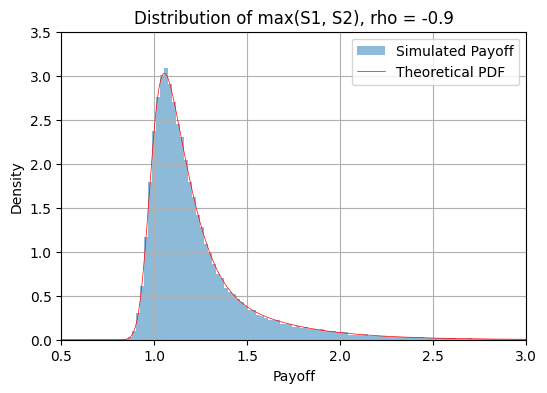
\includegraphics[width=0.49\textwidth]{Exercise_set_02/img/04_rho_neg.png}
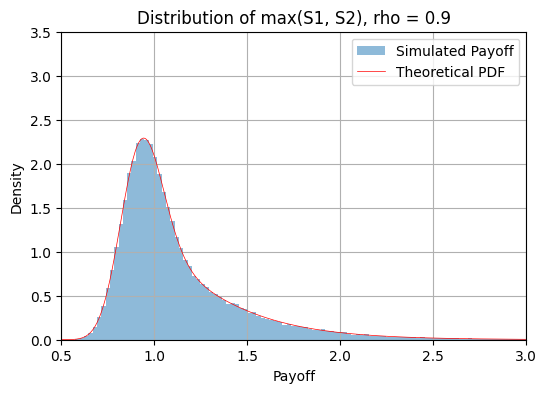
\includegraphics[width=0.49\textwidth]{Exercise_set_02/img/04_rho_pos.png}
\caption{Histogram of simulated $\max(S_1, S_2)$ for $\rho = -0.9$ (left) and $\rho = 0.9$ (right).}
\end{figure}

The sample mean and variance were calculated, and a $95\%$ confidence interval for the expected payoff was constructed using the central limit theorem.

\begin{center}
\begin{tabular}{|c|c|c|c|c|c|}
\hline
$\rho$ & Sample Mean & 95\% CI & Sample Variance & Theor. Mean & Theor. Variance \\
\hline
$-0.9$ & 1.2228 & [1.2210,\;1.2245] & 0.0821 & 1.2219 & 0.0585 \\
\hline
$+0.9$ & 1.1187 & [1.1166,\;1.1208] & 0.1133 & 1.1160 & 0.0852 \\
\hline
\end{tabular}
\end{center}

The simulation confirms that negative correlation increases the spread of possible outcomes, resulting in a higher average maximum. Positive correlation concentrates the joint distribution, lowering both the variance and the expected value of the maximum.

\begin{thebibliography}{1}
\bibitem{nadarajah2008}
S.~Nadarajah and S.~Kotz, ``Exact Distribution of the Max/Min of Two Gaussian Random Variables,'' \emph{IEEE Transactions on VLSI Systems}, vol.~16, no.~2, pp.~210--212, 2008.
\end{thebibliography}

\newpage

\end{document}
